\documentclass[1p]{elsarticle_modified}
%\bibliographystyle{elsarticle-num}

%\usepackage[colorlinks]{hyperref}
%\usepackage{abbrmath_seonhwa} %\Abb, \Ascr, \Acal ,\Abf, \Afrak
\usepackage{amsfonts}
\usepackage{amssymb}
\usepackage{amsmath}
\usepackage{amsthm}
\usepackage{scalefnt}
\usepackage{amsbsy}
\usepackage{kotex}
\usepackage{caption}
\usepackage{subfig}
\usepackage{color}
\usepackage{graphicx}
\usepackage{xcolor} %% white, black, red, green, blue, cyan, magenta, yellow
\usepackage{float}
\usepackage{setspace}
\usepackage{hyperref}

\usepackage{tikz}
\usetikzlibrary{arrows}

\usepackage{multirow}
\usepackage{array} % fixed length table
\usepackage{hhline}

%%%%%%%%%%%%%%%%%%%%%
\makeatletter
\renewcommand*\env@matrix[1][\arraystretch]{%
	\edef\arraystretch{#1}%
	\hskip -\arraycolsep
	\let\@ifnextchar\new@ifnextchar
	\array{*\c@MaxMatrixCols c}}
\makeatother %https://tex.stackexchange.com/questions/14071/how-can-i-increase-the-line-spacing-in-a-matrix
%%%%%%%%%%%%%%%

\usepackage[normalem]{ulem}

\newcommand{\msout}[1]{\ifmmode\text{\sout{\ensuremath{#1}}}\else\sout{#1}\fi}
%SOURCE: \msout is \stkout macro in https://tex.stackexchange.com/questions/20609/strikeout-in-math-mode

\newcommand{\cancel}[1]{
	\ifmmode
	{\color{red}\msout{#1}}
	\else
	{\color{red}\sout{#1}}
	\fi
}

\newcommand{\add}[1]{
	{\color{blue}\uwave{#1}}
}

\newcommand{\replace}[2]{
	\ifmmode
	{\color{red}\msout{#1}}{\color{blue}\uwave{#2}}
	\else
	{\color{red}\sout{#1}}{\color{blue}\uwave{#2}}
	\fi
}

\newcommand{\Sol}{\mathcal{S}} %segment
\newcommand{\D}{D} %diagram
\newcommand{\A}{\mathcal{A}} %arc


%%%%%%%%%%%%%%%%%%%%%%%%%%%%%5 test

\def\sl{\operatorname{\textup{SL}}(2,\Cbb)}
\def\psl{\operatorname{\textup{PSL}}(2,\Cbb)}
\def\quan{\mkern 1mu \triangleright \mkern 1mu}

\theoremstyle{definition}
\newtheorem{thm}{Theorem}[section]
\newtheorem{prop}[thm]{Proposition}
\newtheorem{lem}[thm]{Lemma}
\newtheorem{ques}[thm]{Question}
\newtheorem{cor}[thm]{Corollary}
\newtheorem{defn}[thm]{Definition}
\newtheorem{exam}[thm]{Example}
\newtheorem{rmk}[thm]{Remark}
\newtheorem{alg}[thm]{Algorithm}

\newcommand{\I}{\sqrt{-1}}
\begin{document}

%\begin{frontmatter}
%
%\title{Boundary parabolic representations of knots up to 8 crossings}
%
%%% Group authors per affiliation:
%\author{Yunhi Cho} 
%\address{Department of Mathematics, University of Seoul, Seoul, Korea}
%\ead{yhcho@uos.ac.kr}
%
%
%\author{Seonhwa Kim} %\fnref{s_kim}}
%\address{Center for Geometry and Physics, Institute for Basic Science, Pohang, 37673, Korea}
%\ead{ryeona17@ibs.re.kr}
%
%\author{Hyuk Kim}
%\address{Department of Mathematical Sciences, Seoul National University, Seoul 08826, Korea}
%\ead{hyukkim@snu.ac.kr}
%
%\author{Seokbeom Yoon}
%\address{Department of Mathematical Sciences, Seoul National University, Seoul, 08826,  Korea}
%\ead{sbyoon15@snu.ac.kr}
%
%\begin{abstract}
%We find all boundary parabolic representation of knots up to 8 crossings.
%
%\end{abstract}
%\begin{keyword}
%    \MSC[2010] 57M25 
%\end{keyword}
%
%\end{frontmatter}

%\linenumbers
%\tableofcontents
%
\newcommand\colored[1]{\textcolor{white}{\rule[-0.35ex]{0.8em}{1.4ex}}\kern-0.8em\color{red} #1}%
%\newcommand\colored[1]{\textcolor{white}{ #1}\kern-2.17ex	\textcolor{white}{ #1}\kern-1.81ex	\textcolor{white}{ #1}\kern-2.15ex\color{red}#1	}

{\Large $\underline{11n_{168}~(K11n_{168})}$}

\setlength{\tabcolsep}{10pt}
\renewcommand{\arraystretch}{1.6}
\vspace{1cm}\begin{tabular}{m{100pt}>{\centering\arraybackslash}m{274pt}}
\multirow{5}{120pt}{
	\centering
	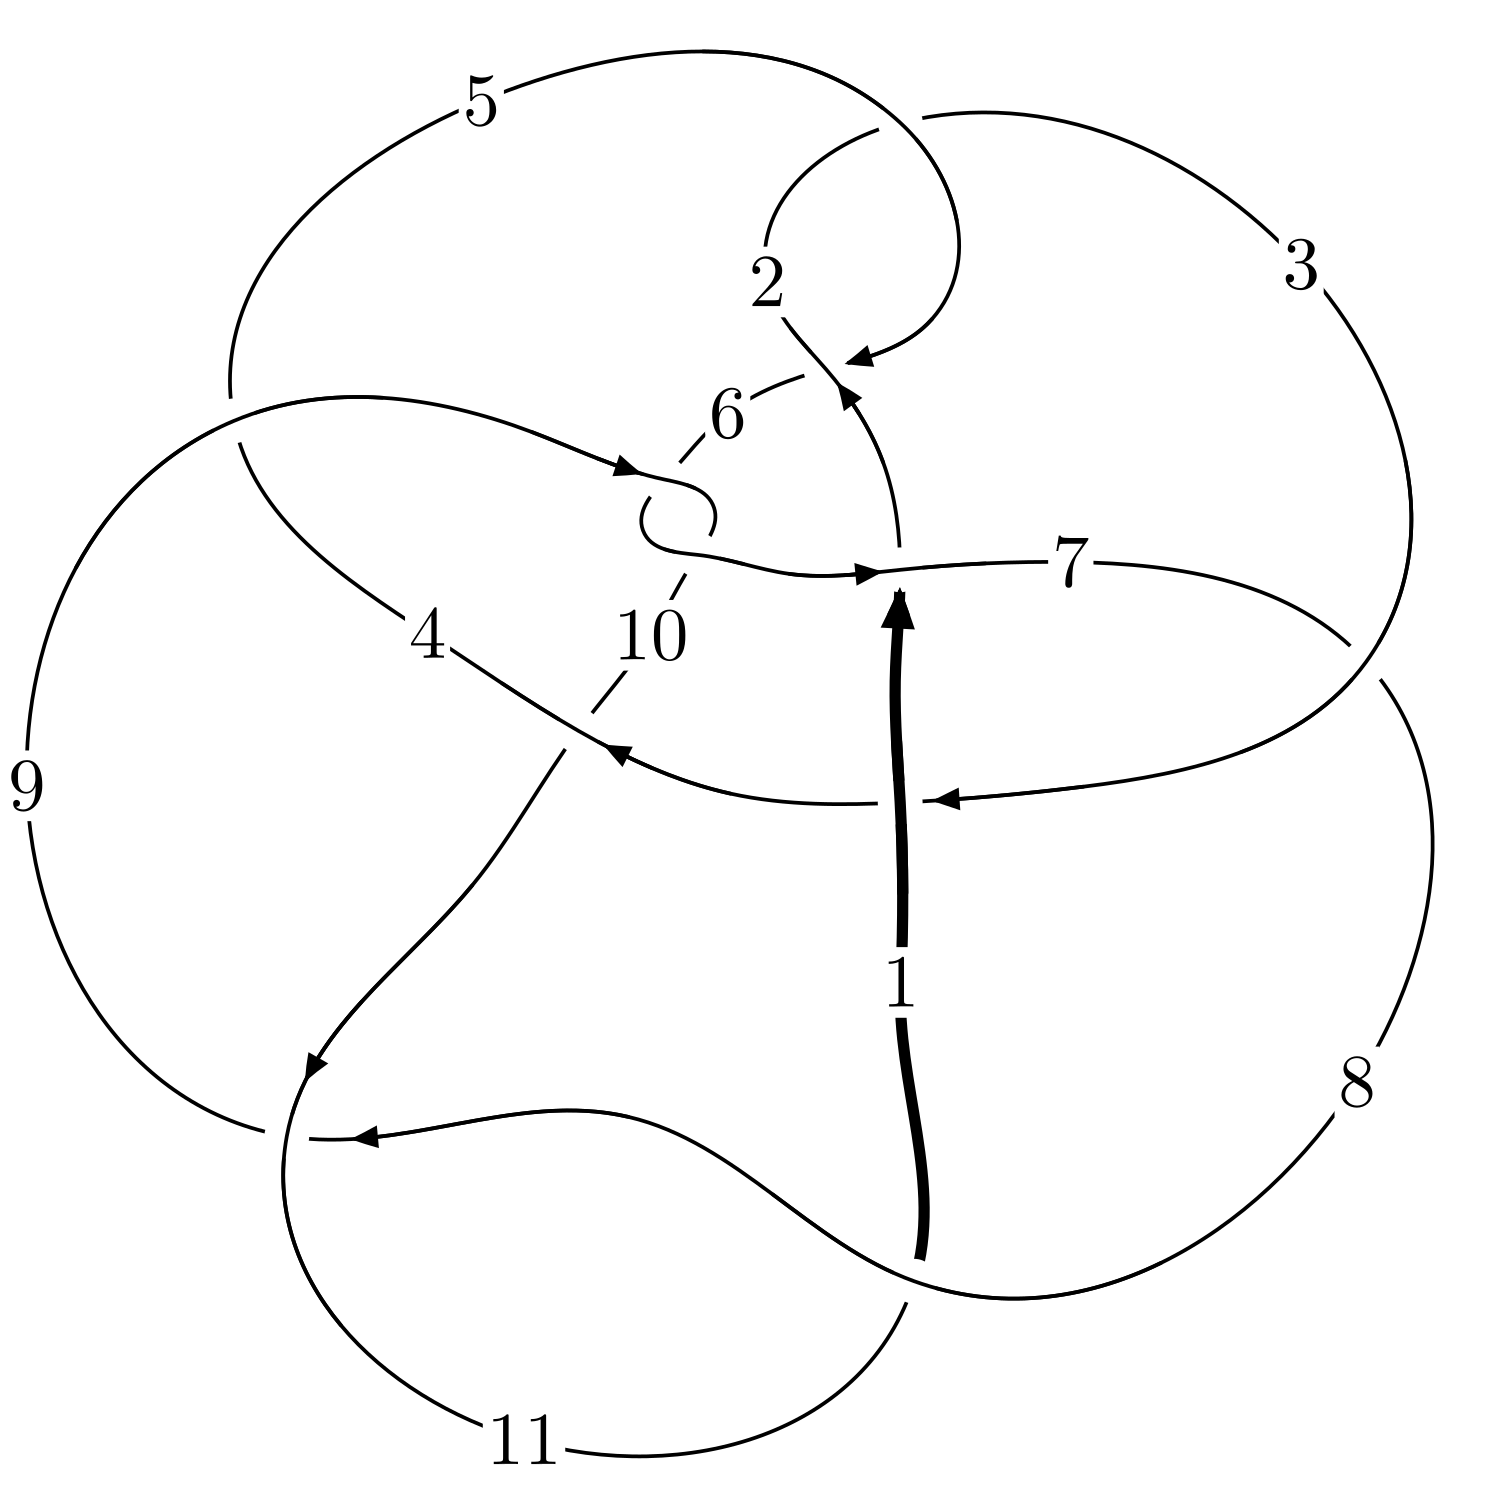
\includegraphics[width=112pt]{../../../GIT/diagram.site/Diagrams/png/784_11n_168.png}\\
\ \ \ A knot diagram\footnotemark}&
\allowdisplaybreaks
\textbf{Linearized knot diagam} \\
\cline{2-2}
 &
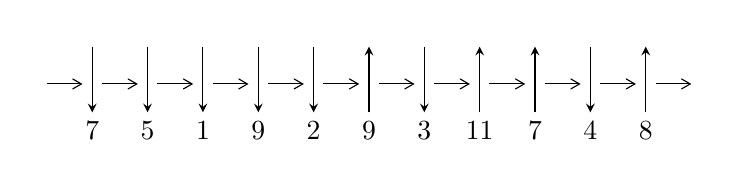
\begin{tikzpicture}[x=20pt, y=17pt]
	% nodes
	\node (C0) at (0, 0) {};
	\node (C1) at (1, 0) {};
	\node (C1U) at (1, +1) {};
	\node (C1D) at (1, -1) {7};

	\node (C2) at (2, 0) {};
	\node (C2U) at (2, +1) {};
	\node (C2D) at (2, -1) {5};

	\node (C3) at (3, 0) {};
	\node (C3U) at (3, +1) {};
	\node (C3D) at (3, -1) {1};

	\node (C4) at (4, 0) {};
	\node (C4U) at (4, +1) {};
	\node (C4D) at (4, -1) {9};

	\node (C5) at (5, 0) {};
	\node (C5U) at (5, +1) {};
	\node (C5D) at (5, -1) {2};

	\node (C6) at (6, 0) {};
	\node (C6U) at (6, +1) {};
	\node (C6D) at (6, -1) {9};

	\node (C7) at (7, 0) {};
	\node (C7U) at (7, +1) {};
	\node (C7D) at (7, -1) {3};

	\node (C8) at (8, 0) {};
	\node (C8U) at (8, +1) {};
	\node (C8D) at (8, -1) {11};

	\node (C9) at (9, 0) {};
	\node (C9U) at (9, +1) {};
	\node (C9D) at (9, -1) {7};

	\node (C10) at (10, 0) {};
	\node (C10U) at (10, +1) {};
	\node (C10D) at (10, -1) {4};

	\node (C11) at (11, 0) {};
	\node (C11U) at (11, +1) {};
	\node (C11D) at (11, -1) {8};
	\node (C12) at (12, 0) {};

	% arrows
	\draw[->,>={angle 60}]
	(C0) edge (C1) (C1) edge (C2) (C2) edge (C3) (C3) edge (C4) (C4) edge (C5) (C5) edge (C6) (C6) edge (C7) (C7) edge (C8) (C8) edge (C9) (C9) edge (C10) (C10) edge (C11) (C11) edge (C12) ;	\draw[->,>=stealth]
	(C1U) edge (C1D) (C2U) edge (C2D) (C3U) edge (C3D) (C4U) edge (C4D) (C5U) edge (C5D) (C6D) edge (C6U) (C7U) edge (C7D) (C8D) edge (C8U) (C9D) edge (C9U) (C10U) edge (C10D) (C11D) edge (C11U) ;
	\end{tikzpicture} \\
\hhline{~~} \\& 
\textbf{Solving Sequence} \\ \cline{2-2} 
 &
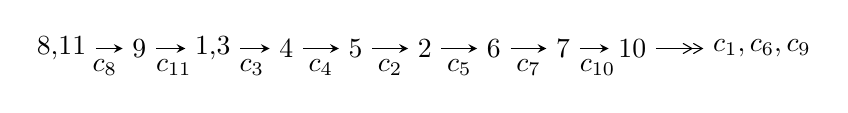
\begin{tikzpicture}[x=25pt, y=7pt]
	% node
	\node (A0) at (-1/8, 0) {8,11};
	\node (A1) at (1, 0) {9};
	\node (A2) at (33/16, 0) {1,3};
	\node (A3) at (25/8, 0) {4};
	\node (A4) at (33/8, 0) {5};
	\node (A5) at (41/8, 0) {2};
	\node (A6) at (49/8, 0) {6};
	\node (A7) at (57/8, 0) {7};
	\node (A8) at (65/8, 0) {10};
	\node (C1) at (1/2, -1) {$c_{8}$};
	\node (C2) at (3/2, -1) {$c_{11}$};
	\node (C3) at (21/8, -1) {$c_{3}$};
	\node (C4) at (29/8, -1) {$c_{4}$};
	\node (C5) at (37/8, -1) {$c_{2}$};
	\node (C6) at (45/8, -1) {$c_{5}$};
	\node (C7) at (53/8, -1) {$c_{7}$};
	\node (C8) at (61/8, -1) {$c_{10}$};
	\node (A9) at (10, 0) {$c_{1},c_{6},c_{9}$};

	% edge
	\draw[->,>=stealth]	
	(A0) edge (A1) (A1) edge (A2) (A2) edge (A3) (A3) edge (A4) (A4) edge (A5) (A5) edge (A6) (A6) edge (A7) (A7) edge (A8) ;
	\draw[->>,>={angle 60}]	
	(A8) edge (A9);
\end{tikzpicture} \\ 

\end{tabular} \\

\footnotetext{
The image of knot diagram is generated by the software ``\textbf{Draw programme}" developed by Andrew Bartholomew(\url{http://www.layer8.co.uk/maths/draw/index.htm\#Running-draw}), where we modified some parts for our purpose(\url{https://github.com/CATsTAILs/LinksPainter}).
}\phantom \\ \newline 
\centering \textbf{Ideals for irreducible components\footnotemark of $X_{\text{par}}$} 
 
\begin{align*}
I^u_{1}&=\langle 
115868 u^{24}-821040 u^{23}+\cdots+306031 b-602429,\\
\phantom{I^u_{1}}&\phantom{= \langle  }1065901 u^{24}-8567064 u^{23}+\cdots+1224124 a+13420127,\;u^{25}-8 u^{24}+\cdots+55 u-4\rangle \\
I^u_{2}&=\langle 
- u^{11} a- u^{11}+\cdots+b- a,\;u^{10} a+3 u^{11}+\cdots+a-9,\\
\phantom{I^u_{2}}&\phantom{= \langle  }u^{12}+3 u^{11}+9 u^{10}+16 u^9+25 u^8+30 u^7+28 u^6+22 u^5+10 u^4+3 u^3- u^2-2 u+1\rangle \\
I^u_{3}&=\langle 
u^{11}+4 u^{10}+11 u^9+22 u^8+35 u^7+47 u^6+52 u^5+48 u^4+37 u^3+22 u^2+b+10 u+2,\\
\phantom{I^u_{3}}&\phantom{= \langle  }3 u^{11}+15 u^{10}+43 u^9+91 u^8+151 u^7+210 u^6+247 u^5+242 u^4+199 u^3+133 u^2+5 a+66 u+20,\\
\phantom{I^u_{3}}&\phantom{= \langle  }u^{12}+5 u^{11}+16 u^{10}+37 u^9+67 u^8+100 u^7+124 u^6+129 u^5+113 u^4+81 u^3+47 u^2+20 u+5\rangle \\
\\
\end{align*}
\raggedright * 3 irreducible components of $\dim_{\mathbb{C}}=0$, with total 61 representations.\\
\footnotetext{All coefficients of polynomials are rational numbers. But the coefficients are sometimes approximated in decimal forms when there is not enough margin.}
\newpage
\renewcommand{\arraystretch}{1}
\centering \section*{I. $I^u_{1}= \langle 1.16\times10^{5} u^{24}-8.21\times10^{5} u^{23}+\cdots+3.06\times10^{5} b-6.02\times10^{5},\;1.07\times10^{6} u^{24}-8.57\times10^{6} u^{23}+\cdots+1.22\times10^{6} a+1.34\times10^{7},\;u^{25}-8 u^{24}+\cdots+55 u-4 \rangle$}
\flushleft \textbf{(i) Arc colorings}\\
\begin{tabular}{m{7pt} m{180pt} m{7pt} m{180pt} }
\flushright $a_{8}=$&$\begin{pmatrix}1\\0\end{pmatrix}$ \\
\flushright $a_{11}=$&$\begin{pmatrix}0\\u\end{pmatrix}$ \\
\flushright $a_{9}=$&$\begin{pmatrix}1\\- u^2\end{pmatrix}$ \\
\flushright $a_{1}=$&$\begin{pmatrix}u\\u\end{pmatrix}$ \\
\flushright $a_{3}=$&$\begin{pmatrix}-0.870746 u^{24}+6.99853 u^{23}+\cdots+87.0860 u-10.9630\\-0.378615 u^{24}+2.68287 u^{23}+\cdots-14.1356 u+1.96852\end{pmatrix}$ \\
\flushright $a_{4}=$&$\begin{pmatrix}-0.524689 u^{24}+3.93260 u^{23}+\cdots+64.2937 u-9.44858\\-0.0325588 u^{24}-0.383056 u^{23}+\cdots-36.9280 u+3.48298\end{pmatrix}$ \\
\flushright $a_{5}=$&$\begin{pmatrix}-0.768694 u^{24}+5.93994 u^{23}+\cdots+88.7503 u-11.8719\\-0.398251 u^{24}+1.85942 u^{23}+\cdots-32.9107 u+3.26180\end{pmatrix}$ \\
\flushright $a_{2}=$&$\begin{pmatrix}-1.38249 u^{24}+10.8931 u^{23}+\cdots+95.0899 u-8.66735\\-0.943676 u^{24}+6.44578 u^{23}+\cdots-15.9909 u+1.92923\end{pmatrix}$ \\
\flushright $a_{6}=$&$\begin{pmatrix}-0.221379 u^{24}+2.09877 u^{23}+\cdots+51.1671 u-7.44194\\-0.205861 u^{24}+1.51059 u^{23}+\cdots+6.56495 u-0.0489787\end{pmatrix}$ \\
\flushright $a_{7}=$&$\begin{pmatrix}0.308644 u^{24}-2.51950 u^{23}+\cdots-38.8206 u+6.17994\\0.0434891 u^{24}-0.354768 u^{23}+\cdots+8.34298 u-1.06062\end{pmatrix}$ \\
\flushright $a_{10}=$&$\begin{pmatrix}0.125366 u^{24}-0.975163 u^{23}+\cdots-16.9600 u+3.39492\\-0.190134 u^{24}+1.63610 u^{23}+\cdots+19.4081 u-1.61106\end{pmatrix}$\\ \flushright $a_{10}=$&$\begin{pmatrix}0.125366 u^{24}-0.975163 u^{23}+\cdots-16.9600 u+3.39492\\-0.190134 u^{24}+1.63610 u^{23}+\cdots+19.4081 u-1.61106\end{pmatrix}$\\&\end{tabular}
\flushleft \textbf{(ii) Obstruction class $= -1$}\\~\\
\flushleft \textbf{(iii) Cusp Shapes $= \frac{23011}{27821} u^{24}-\frac{191892}{27821} u^{23}+\cdots-\frac{108563}{27821} u-\frac{344142}{27821}$}\\~\\
\newpage\renewcommand{\arraystretch}{1}
\flushleft \textbf{(iv) u-Polynomials at the component}\newline \\
\begin{tabular}{m{50pt}|m{274pt}}
Crossings & \hspace{64pt}u-Polynomials at each crossing \\
\hline $$\begin{aligned}c_{1}\end{aligned}$$&$\begin{aligned}
&u^{25}+22 u^{24}+\cdots+40960 u+4096
\end{aligned}$\\
\hline $$\begin{aligned}c_{2},c_{5}\end{aligned}$$&$\begin{aligned}
&u^{25}-8 u^{24}+\cdots-3 u+2
\end{aligned}$\\
\hline $$\begin{aligned}c_{3},c_{7}\end{aligned}$$&$\begin{aligned}
&u^{25}-7 u^{23}+\cdots-8 u+1
\end{aligned}$\\
\hline $$\begin{aligned}c_{4}\end{aligned}$$&$\begin{aligned}
&u^{25}- u^{24}+\cdots-80 u+85
\end{aligned}$\\
\hline $$\begin{aligned}c_{6},c_{9}\end{aligned}$$&$\begin{aligned}
&u^{25}+15 u^{23}+\cdots- u+1
\end{aligned}$\\
\hline $$\begin{aligned}c_{8},c_{11}\end{aligned}$$&$\begin{aligned}
&u^{25}+8 u^{24}+\cdots+55 u+4
\end{aligned}$\\
\hline $$\begin{aligned}c_{10}\end{aligned}$$&$\begin{aligned}
&u^{25}-8 u^{23}+\cdots-18 u+28
\end{aligned}$\\
\hline
\end{tabular}\\~\\
\newpage\renewcommand{\arraystretch}{1}
\flushleft \textbf{(v) Riley Polynomials at the component}\newline \\
\begin{tabular}{m{50pt}|m{274pt}}
Crossings & \hspace{64pt}Riley Polynomials at each crossing \\
\hline $$\begin{aligned}c_{1}\end{aligned}$$&$\begin{aligned}
&y^{25}-4 y^{24}+\cdots+92274688 y-16777216
\end{aligned}$\\
\hline $$\begin{aligned}c_{2},c_{5}\end{aligned}$$&$\begin{aligned}
&y^{25}+8 y^{24}+\cdots-51 y-4
\end{aligned}$\\
\hline $$\begin{aligned}c_{3},c_{7}\end{aligned}$$&$\begin{aligned}
&y^{25}-14 y^{24}+\cdots+22 y-1
\end{aligned}$\\
\hline $$\begin{aligned}c_{4}\end{aligned}$$&$\begin{aligned}
&y^{25}-23 y^{24}+\cdots+73550 y-7225
\end{aligned}$\\
\hline $$\begin{aligned}c_{6},c_{9}\end{aligned}$$&$\begin{aligned}
&y^{25}+30 y^{24}+\cdots+3 y-1
\end{aligned}$\\
\hline $$\begin{aligned}c_{8},c_{11}\end{aligned}$$&$\begin{aligned}
&y^{25}+16 y^{24}+\cdots+753 y-16
\end{aligned}$\\
\hline $$\begin{aligned}c_{10}\end{aligned}$$&$\begin{aligned}
&y^{25}-16 y^{24}+\cdots+4188 y-784
\end{aligned}$\\
\hline
\end{tabular}\\~\\
\newpage\flushleft \textbf{(vi) Complex Volumes and Cusp Shapes}
$$\begin{array}{c|c|c}  
\text{Solutions to }I^u_{1}& \I (\text{vol} + \sqrt{-1}CS) & \text{Cusp shape}\\
 \hline 
\begin{aligned}
u &= \phantom{-}1.000760 + 0.214781 I \\
a &= \phantom{-}0.181546 + 0.179308 I \\
b &= \phantom{-}1.019350 - 0.663007 I\end{aligned}
 & -4.81720 + 2.41116 I & -4.79174 - 2.48268 I \\ \hline\begin{aligned}
u &= \phantom{-}1.000760 - 0.214781 I \\
a &= \phantom{-}0.181546 - 0.179308 I \\
b &= \phantom{-}1.019350 + 0.663007 I\end{aligned}
 & -4.81720 - 2.41116 I & -4.79174 + 2.48268 I \\ \hline\begin{aligned}
u &= -1.012850 + 0.261202 I \\
a &= -0.316874 + 0.202205 I \\
b &= -0.149236 + 0.123502 I\end{aligned}
 & \phantom{-}1.91022 - 0.92265 I & \phantom{-}6.06720 + 6.51070 I \\ \hline\begin{aligned}
u &= -1.012850 - 0.261202 I \\
a &= -0.316874 - 0.202205 I \\
b &= -0.149236 - 0.123502 I\end{aligned}
 & \phantom{-}1.91022 + 0.92265 I & \phantom{-}6.06720 - 6.51070 I \\ \hline\begin{aligned}
u &= \phantom{-}0.041993 + 0.934875 I \\
a &= \phantom{-}1.48887 + 0.80671 I \\
b &= \phantom{-}1.113720 - 0.401444 I\end{aligned}
 & -3.12369 + 0.06362 I & -5.51965 + 0.12740 I \\ \hline\begin{aligned}
u &= \phantom{-}0.041993 - 0.934875 I \\
a &= \phantom{-}1.48887 - 0.80671 I \\
b &= \phantom{-}1.113720 + 0.401444 I\end{aligned}
 & -3.12369 - 0.06362 I & -5.51965 - 0.12740 I \\ \hline\begin{aligned}
u &= \phantom{-}0.011472 + 1.113580 I \\
a &= \phantom{-}1.64705 + 0.28486 I \\
b &= \phantom{-}1.055800 - 0.669349 I\end{aligned}
 & -3.62398 + 0.55768 I & -7.12692 - 1.89809 I \\ \hline\begin{aligned}
u &= \phantom{-}0.011472 - 1.113580 I \\
a &= \phantom{-}1.64705 - 0.28486 I \\
b &= \phantom{-}1.055800 + 0.669349 I\end{aligned}
 & -3.62398 - 0.55768 I & -7.12692 + 1.89809 I \\ \hline\begin{aligned}
u &= \phantom{-}0.247489 + 1.108210 I \\
a &= -1.82938 - 0.09919 I \\
b &= -1.12346 + 1.07222 I\end{aligned}
 & \phantom{-}1.38725 + 4.87941 I & -6.34329 + 0.12140 I \\ \hline\begin{aligned}
u &= \phantom{-}0.247489 - 1.108210 I \\
a &= -1.82938 + 0.09919 I \\
b &= -1.12346 - 1.07222 I\end{aligned}
 & \phantom{-}1.38725 - 4.87941 I & -6.34329 - 0.12140 I\\
 \hline 
 \end{array}$$\newpage$$\begin{array}{c|c|c}  
\text{Solutions to }I^u_{1}& \I (\text{vol} + \sqrt{-1}CS) & \text{Cusp shape}\\
 \hline 
\begin{aligned}
u &= \phantom{-}1.168910 + 0.049676 I \\
a &= -0.170031 + 0.065726 I \\
b &= -0.991209 + 0.696352 I\end{aligned}
 & -4.29953 + 9.06645 I & -3.72304 - 7.02542 I \\ \hline\begin{aligned}
u &= \phantom{-}1.168910 - 0.049676 I \\
a &= -0.170031 - 0.065726 I \\
b &= -0.991209 - 0.696352 I\end{aligned}
 & -4.29953 - 9.06645 I & -3.72304 + 7.02542 I \\ \hline\begin{aligned}
u &= -0.159099 + 1.201110 I \\
a &= -1.015220 - 0.149383 I \\
b &= -0.657268 + 0.350420 I\end{aligned}
 & -1.98209 - 2.65903 I & -3.09005 + 4.34714 I \\ \hline\begin{aligned}
u &= -0.159099 - 1.201110 I \\
a &= -1.015220 + 0.149383 I \\
b &= -0.657268 - 0.350420 I\end{aligned}
 & -1.98209 + 2.65903 I & -3.09005 - 4.34714 I \\ \hline\begin{aligned}
u &= \phantom{-}0.442257 + 0.365564 I \\
a &= \phantom{-}1.133650 - 0.436737 I \\
b &= -0.647135 - 0.820882 I\end{aligned}
 & \phantom{-}3.61375 - 2.05944 I & -4.90254 + 7.19693 I \\ \hline\begin{aligned}
u &= \phantom{-}0.442257 - 0.365564 I \\
a &= \phantom{-}1.133650 + 0.436737 I \\
b &= -0.647135 + 0.820882 I\end{aligned}
 & \phantom{-}3.61375 + 2.05944 I & -4.90254 - 7.19693 I \\ \hline\begin{aligned}
u &= \phantom{-}0.42788 + 1.38215 I \\
a &= \phantom{-}1.70744 + 0.14723 I \\
b &= \phantom{-}1.36183 - 0.94506 I\end{aligned}
 & -9.79096 + 7.40216 I & -7.26136 - 3.90619 I \\ \hline\begin{aligned}
u &= \phantom{-}0.42788 - 1.38215 I \\
a &= \phantom{-}1.70744 - 0.14723 I \\
b &= \phantom{-}1.36183 + 0.94506 I\end{aligned}
 & -9.79096 - 7.40216 I & -7.26136 + 3.90619 I \\ \hline\begin{aligned}
u &= \phantom{-}0.53216 + 1.39760 I \\
a &= -1.63900 - 0.14616 I \\
b &= -1.38003 + 0.93988 I\end{aligned}
 & -8.8717 + 15.0132 I & -5.71790 - 7.82964 I \\ \hline\begin{aligned}
u &= \phantom{-}0.53216 - 1.39760 I \\
a &= -1.63900 + 0.14616 I \\
b &= -1.38003 - 0.93988 I\end{aligned}
 & -8.8717 - 15.0132 I & -5.71790 + 7.82964 I\\
 \hline 
 \end{array}$$\newpage$$\begin{array}{c|c|c}  
\text{Solutions to }I^u_{1}& \I (\text{vol} + \sqrt{-1}CS) & \text{Cusp shape}\\
 \hline 
\begin{aligned}
u &= \phantom{-}0.68747 + 1.33439 I \\
a &= \phantom{-}0.628461 + 0.691868 I \\
b &= \phantom{-}1.015420 + 0.130266 I\end{aligned}
 & -7.96688 + 3.80546 I & -9.00823 - 2.72232 I \\ \hline\begin{aligned}
u &= \phantom{-}0.68747 - 1.33439 I \\
a &= \phantom{-}0.628461 - 0.691868 I \\
b &= \phantom{-}1.015420 - 0.130266 I\end{aligned}
 & -7.96688 - 3.80546 I & -9.00823 + 2.72232 I \\ \hline\begin{aligned}
u &= \phantom{-}0.54107 + 1.49661 I \\
a &= -0.679365 - 0.581046 I \\
b &= -0.907003 - 0.057306 I\end{aligned}
 & -8.86649 - 2.64359 I & -10.06958 + 2.50086 I \\ \hline\begin{aligned}
u &= \phantom{-}0.54107 - 1.49661 I \\
a &= -0.679365 + 0.581046 I \\
b &= -0.907003 + 0.057306 I\end{aligned}
 & -8.86649 + 2.64359 I & -10.06958 - 2.50086 I \\ \hline\begin{aligned}
u &= \phantom{-}0.140989\phantom{ +0.000000I} \\
a &= -3.52430\phantom{ +0.000000I} \\
b &= \phantom{-}0.578442\phantom{ +0.000000I}\end{aligned}
 & -0.898624\phantom{ +0.000000I} & -11.0260\phantom{ +0.000000I}\\
 \hline 
 \end{array}$$\newpage\newpage\renewcommand{\arraystretch}{1}
\centering \section*{II. $I^u_{2}= \langle - u^{11} a- u^{11}+\cdots+b- a,\;u^{10} a+3 u^{11}+\cdots+a-9,\;u^{12}+3 u^{11}+\cdots-2 u+1 \rangle$}
\flushleft \textbf{(i) Arc colorings}\\
\begin{tabular}{m{7pt} m{180pt} m{7pt} m{180pt} }
\flushright $a_{8}=$&$\begin{pmatrix}1\\0\end{pmatrix}$ \\
\flushright $a_{11}=$&$\begin{pmatrix}0\\u\end{pmatrix}$ \\
\flushright $a_{9}=$&$\begin{pmatrix}1\\- u^2\end{pmatrix}$ \\
\flushright $a_{1}=$&$\begin{pmatrix}u\\u\end{pmatrix}$ \\
\flushright $a_{3}=$&$\begin{pmatrix}a\\u^{11} a+u^{11}+\cdots-2 a u+a\end{pmatrix}$ \\
\flushright $a_{4}=$&$\begin{pmatrix}- u^{11} a-2 u^{10} a+\cdots+3 a u+u\\u^{11}+4 u^{10}+\cdots+a u+u\end{pmatrix}$ \\
\flushright $a_{5}=$&$\begin{pmatrix}u^{10}+2 u^9+\cdots+a+1\\- u^{11} a+u^{11}+\cdots- a+u\end{pmatrix}$ \\
\flushright $a_{2}=$&$\begin{pmatrix}u^9 a- u^{10}+\cdots+a-2\\- u^{11}-4 u^{10}+\cdots+a+2 u\end{pmatrix}$ \\
\flushright $a_{6}=$&$\begin{pmatrix}u^{11} a+2 u^{10} a+\cdots- u+3\\u^{11}+4 u^{10}+\cdots-2 a- u\end{pmatrix}$ \\
\flushright $a_{7}=$&$\begin{pmatrix}u^9 a- u^{10}+\cdots+a-2\\- u^{11}-4 u^{10}+\cdots+a+u\end{pmatrix}$ \\
\flushright $a_{10}=$&$\begin{pmatrix}-2 u^{11} a-6 u^{10} a+\cdots- a+2\\- u^{11} a+u^{11}+\cdots- a+5 u\end{pmatrix}$\\ \flushright $a_{10}=$&$\begin{pmatrix}-2 u^{11} a-6 u^{10} a+\cdots- a+2\\- u^{11} a+u^{11}+\cdots- a+5 u\end{pmatrix}$\\&\end{tabular}
\flushleft \textbf{(ii) Obstruction class $= -1$}\\~\\
\flushleft \textbf{(iii) Cusp Shapes $= 4 u^{11}+4 u^{10}+12 u^9-4 u^7-20 u^6-28 u^5-12 u^4-8 u^3+12 u^2+8 u-6$}\\~\\
\newpage\renewcommand{\arraystretch}{1}
\flushleft \textbf{(iv) u-Polynomials at the component}\newline \\
\begin{tabular}{m{50pt}|m{274pt}}
Crossings & \hspace{64pt}u-Polynomials at each crossing \\
\hline $$\begin{aligned}c_{1}\end{aligned}$$&$\begin{aligned}
&(u-1)^{24}
\end{aligned}$\\
\hline $$\begin{aligned}c_{2},c_{5}\end{aligned}$$&$\begin{aligned}
&(u^{12}+5 u^{11}+\cdots+3 u^2+1)^{2}
\end{aligned}$\\
\hline $$\begin{aligned}c_{3},c_{7}\end{aligned}$$&$\begin{aligned}
&u^{24}- u^{23}+\cdots-4 u+1
\end{aligned}$\\
\hline $$\begin{aligned}c_{4}\end{aligned}$$&$\begin{aligned}
&u^{24}+u^{23}+\cdots+162 u+27
\end{aligned}$\\
\hline $$\begin{aligned}c_{6},c_{9}\end{aligned}$$&$\begin{aligned}
&u^{24}+3 u^{23}+\cdots+400 u+109
\end{aligned}$\\
\hline $$\begin{aligned}c_{8},c_{11}\end{aligned}$$&$\begin{aligned}
&(u^{12}-3 u^{11}+\cdots+2 u+1)^{2}
\end{aligned}$\\
\hline $$\begin{aligned}c_{10}\end{aligned}$$&$\begin{aligned}
&u^{24}+u^{23}+\cdots-774 u+135
\end{aligned}$\\
\hline
\end{tabular}\\~\\
\newpage\renewcommand{\arraystretch}{1}
\flushleft \textbf{(v) Riley Polynomials at the component}\newline \\
\begin{tabular}{m{50pt}|m{274pt}}
Crossings & \hspace{64pt}Riley Polynomials at each crossing \\
\hline $$\begin{aligned}c_{1}\end{aligned}$$&$\begin{aligned}
&(y-1)^{24}
\end{aligned}$\\
\hline $$\begin{aligned}c_{2},c_{5}\end{aligned}$$&$\begin{aligned}
&(y^{12}+y^{11}+\cdots+6 y+1)^{2}
\end{aligned}$\\
\hline $$\begin{aligned}c_{3},c_{7}\end{aligned}$$&$\begin{aligned}
&y^{24}+3 y^{23}+\cdots-8 y+1
\end{aligned}$\\
\hline $$\begin{aligned}c_{4}\end{aligned}$$&$\begin{aligned}
&y^{24}-21 y^{23}+\cdots+93636 y+729
\end{aligned}$\\
\hline $$\begin{aligned}c_{6},c_{9}\end{aligned}$$&$\begin{aligned}
&y^{24}+15 y^{23}+\cdots-39228 y+11881
\end{aligned}$\\
\hline $$\begin{aligned}c_{8},c_{11}\end{aligned}$$&$\begin{aligned}
&(y^{12}+9 y^{11}+\cdots-6 y+1)^{2}
\end{aligned}$\\
\hline $$\begin{aligned}c_{10}\end{aligned}$$&$\begin{aligned}
&y^{24}-17 y^{23}+\cdots-49896 y+18225
\end{aligned}$\\
\hline
\end{tabular}\\~\\
\newpage\flushleft \textbf{(vi) Complex Volumes and Cusp Shapes}
$$\begin{array}{c|c|c}  
\text{Solutions to }I^u_{2}& \I (\text{vol} + \sqrt{-1}CS) & \text{Cusp shape}\\
 \hline 
\begin{aligned}
u &= -1.002830 + 0.154838 I \\
a &= -0.348206 + 0.268306 I \\
b &= -0.387233 - 0.109050 I\end{aligned}
 & \phantom{-}1.93604 - 0.91968 I & \phantom{-}3.53074 + 7.18196 I \\ \hline\begin{aligned}
u &= -1.002830 + 0.154838 I \\
a &= -0.263185 + 0.207938 I \\
b &= \phantom{-}0.097566 + 0.372381 I\end{aligned}
 & \phantom{-}1.93604 - 0.91968 I & \phantom{-}3.53074 + 7.18196 I \\ \hline\begin{aligned}
u &= -1.002830 - 0.154838 I \\
a &= -0.348206 - 0.268306 I \\
b &= -0.387233 + 0.109050 I\end{aligned}
 & \phantom{-}1.93604 + 0.91968 I & \phantom{-}3.53074 - 7.18196 I \\ \hline\begin{aligned}
u &= -1.002830 - 0.154838 I \\
a &= -0.263185 - 0.207938 I \\
b &= \phantom{-}0.097566 - 0.372381 I\end{aligned}
 & \phantom{-}1.93604 + 0.91968 I & \phantom{-}3.53074 - 7.18196 I \\ \hline\begin{aligned}
u &= \phantom{-}0.170454 + 1.138930 I \\
a &= -0.96275 - 1.64559 I \\
b &= -1.07597 - 2.21108 I\end{aligned}
 & -6.29691 + 5.40399 I & -10.52298 - 8.56336 I \\ \hline\begin{aligned}
u &= \phantom{-}0.170454 + 1.138930 I \\
a &= \phantom{-}2.66189 - 0.86518 I \\
b &= \phantom{-}0.624755 - 0.225337 I\end{aligned}
 & -6.29691 + 5.40399 I & -10.52298 - 8.56336 I \\ \hline\begin{aligned}
u &= \phantom{-}0.170454 - 1.138930 I \\
a &= -0.96275 + 1.64559 I \\
b &= -1.07597 + 2.21108 I\end{aligned}
 & -6.29691 - 5.40399 I & -10.52298 + 8.56336 I \\ \hline\begin{aligned}
u &= \phantom{-}0.170454 - 1.138930 I \\
a &= \phantom{-}2.66189 + 0.86518 I \\
b &= \phantom{-}0.624755 + 0.225337 I\end{aligned}
 & -6.29691 - 5.40399 I & -10.52298 + 8.56336 I \\ \hline\begin{aligned}
u &= \phantom{-}0.001213 + 1.239870 I \\
a &= \phantom{-}1.67353 + 1.23840 I \\
b &= \phantom{-}1.63727 + 1.77021 I\end{aligned}
 & -7.81112 - 2.53747 I & -14.4387 + 1.7127 I \\ \hline\begin{aligned}
u &= \phantom{-}0.001213 + 1.239870 I \\
a &= -2.08845 + 1.27481 I \\
b &= -0.659423 - 0.044313 I\end{aligned}
 & -7.81112 - 2.53747 I & -14.4387 + 1.7127 I\\
 \hline 
 \end{array}$$\newpage$$\begin{array}{c|c|c}  
\text{Solutions to }I^u_{2}& \I (\text{vol} + \sqrt{-1}CS) & \text{Cusp shape}\\
 \hline 
\begin{aligned}
u &= \phantom{-}0.001213 - 1.239870 I \\
a &= \phantom{-}1.67353 - 1.23840 I \\
b &= \phantom{-}1.63727 - 1.77021 I\end{aligned}
 & -7.81112 + 2.53747 I & -14.4387 - 1.7127 I \\ \hline\begin{aligned}
u &= \phantom{-}0.001213 - 1.239870 I \\
a &= -2.08845 - 1.27481 I \\
b &= -0.659423 + 0.044313 I\end{aligned}
 & -7.81112 + 2.53747 I & -14.4387 - 1.7127 I \\ \hline\begin{aligned}
u &= -0.521704 + 1.146910 I \\
a &= \phantom{-}0.562645 - 0.435117 I \\
b &= \phantom{-}0.625850 + 0.653229 I\end{aligned}
 & -1.08693 - 4.46082 I & -0.35199 + 4.72827 I \\ \hline\begin{aligned}
u &= -0.521704 + 1.146910 I \\
a &= -1.54745 + 0.17149 I \\
b &= -1.281210 - 0.495305 I\end{aligned}
 & -1.08693 - 4.46082 I & -0.35199 + 4.72827 I \\ \hline\begin{aligned}
u &= -0.521704 - 1.146910 I \\
a &= \phantom{-}0.562645 + 0.435117 I \\
b &= \phantom{-}0.625850 - 0.653229 I\end{aligned}
 & -1.08693 + 4.46082 I & -0.35199 - 4.72827 I \\ \hline\begin{aligned}
u &= -0.521704 - 1.146910 I \\
a &= -1.54745 - 0.17149 I \\
b &= -1.281210 + 0.495305 I\end{aligned}
 & -1.08693 + 4.46082 I & -0.35199 - 4.72827 I \\ \hline\begin{aligned}
u &= -0.47799 + 1.39365 I \\
a &= \phantom{-}1.107670 + 0.201975 I \\
b &= \phantom{-}1.007830 + 0.931272 I\end{aligned}
 & -2.89796 - 6.22910 I & -8.04009 + 11.28166 I \\ \hline\begin{aligned}
u &= -0.47799 + 1.39365 I \\
a &= -1.344630 + 0.364358 I \\
b &= -0.968657 - 0.487749 I\end{aligned}
 & -2.89796 - 6.22910 I & -8.04009 + 11.28166 I \\ \hline\begin{aligned}
u &= -0.47799 - 1.39365 I \\
a &= \phantom{-}1.107670 - 0.201975 I \\
b &= \phantom{-}1.007830 - 0.931272 I\end{aligned}
 & -2.89796 + 6.22910 I & -8.04009 - 11.28166 I \\ \hline\begin{aligned}
u &= -0.47799 - 1.39365 I \\
a &= -1.344630 - 0.364358 I \\
b &= -0.968657 + 0.487749 I\end{aligned}
 & -2.89796 + 6.22910 I & -8.04009 - 11.28166 I\\
 \hline 
 \end{array}$$\newpage$$\begin{array}{c|c|c}  
\text{Solutions to }I^u_{2}& \I (\text{vol} + \sqrt{-1}CS) & \text{Cusp shape}\\
 \hline 
\begin{aligned}
u &= \phantom{-}0.330854 + 0.169612 I \\
a &= \phantom{-}1.68415 - 2.07618 I \\
b &= \phantom{-}0.708011 + 0.906125 I\end{aligned}
 & -3.58234 - 3.33657 I & -2.17703 + 1.92424 I \\ \hline\begin{aligned}
u &= \phantom{-}0.330854 + 0.169612 I \\
a &= -3.63521 - 0.47890 I \\
b &= -0.828793 + 0.821143 I\end{aligned}
 & -3.58234 - 3.33657 I & -2.17703 + 1.92424 I \\ \hline\begin{aligned}
u &= \phantom{-}0.330854 - 0.169612 I \\
a &= \phantom{-}1.68415 + 2.07618 I \\
b &= \phantom{-}0.708011 - 0.906125 I\end{aligned}
 & -3.58234 + 3.33657 I & -2.17703 - 1.92424 I \\ \hline\begin{aligned}
u &= \phantom{-}0.330854 - 0.169612 I \\
a &= -3.63521 + 0.47890 I \\
b &= -0.828793 - 0.821143 I\end{aligned}
 & -3.58234 + 3.33657 I & -2.17703 - 1.92424 I\\
 \hline 
 \end{array}$$\newpage\newpage\renewcommand{\arraystretch}{1}
\centering \section*{III. $I^u_{3}= \langle u^{11}+4 u^{10}+\cdots+b+2,\;3 u^{11}+15 u^{10}+\cdots+5 a+20,\;u^{12}+5 u^{11}+\cdots+20 u+5 \rangle$}
\flushleft \textbf{(i) Arc colorings}\\
\begin{tabular}{m{7pt} m{180pt} m{7pt} m{180pt} }
\flushright $a_{8}=$&$\begin{pmatrix}1\\0\end{pmatrix}$ \\
\flushright $a_{11}=$&$\begin{pmatrix}0\\u\end{pmatrix}$ \\
\flushright $a_{9}=$&$\begin{pmatrix}1\\- u^2\end{pmatrix}$ \\
\flushright $a_{1}=$&$\begin{pmatrix}u\\u\end{pmatrix}$ \\
\flushright $a_{3}=$&$\begin{pmatrix}-\frac{3}{5} u^{11}-3 u^{10}+\cdots-\frac{66}{5} u-4\\- u^{11}-4 u^{10}+\cdots-10 u-2\end{pmatrix}$ \\
\flushright $a_{4}=$&$\begin{pmatrix}\frac{2}{5} u^{11}+2 u^{10}+\cdots+\frac{24}{5} u+1\\u^{10}+4 u^9+\cdots+8 u+3\end{pmatrix}$ \\
\flushright $a_{5}=$&$\begin{pmatrix}\frac{2}{5} u^{11}+2 u^{10}+\cdots-\frac{6}{5} u-2\\u^{10}+4 u^9+\cdots+8 u+3\end{pmatrix}$ \\
\flushright $a_{2}=$&$\begin{pmatrix}-\frac{9}{5} u^{11}-9 u^{10}+\cdots-\frac{173}{5} u-9\\- u^{11}-5 u^{10}+\cdots-10 u-1\end{pmatrix}$ \\
\flushright $a_{6}=$&$\begin{pmatrix}\frac{4}{5} u^{11}+4 u^{10}+\cdots+\frac{43}{5} u+2\\u^{11}+4 u^{10}+\cdots+5 u+1\end{pmatrix}$ \\
\flushright $a_{7}=$&$\begin{pmatrix}\frac{4}{5} u^{11}+4 u^{10}+\cdots+\frac{48}{5} u+3\\u^{11}+4 u^{10}+\cdots+5 u+1\end{pmatrix}$ \\
\flushright $a_{10}=$&$\begin{pmatrix}\frac{1}{5} u^{11}+u^{10}+\cdots+\frac{37}{5} u+2\\- u^2- u-1\end{pmatrix}$\\ \flushright $a_{10}=$&$\begin{pmatrix}\frac{1}{5} u^{11}+u^{10}+\cdots+\frac{37}{5} u+2\\- u^2- u-1\end{pmatrix}$\\&\end{tabular}
\flushleft \textbf{(ii) Obstruction class $= 1$}\\~\\
\flushleft \textbf{(iii) Cusp Shapes $= -4 u^{11}-14 u^{10}-36 u^9-61 u^8-79 u^7-77 u^6-49 u^5-8 u^4+24 u^3+38 u^2+30 u+14$}\\~\\
\newpage\renewcommand{\arraystretch}{1}
\flushleft \textbf{(iv) u-Polynomials at the component}\newline \\
\begin{tabular}{m{50pt}|m{274pt}}
Crossings & \hspace{64pt}u-Polynomials at each crossing \\
\hline $$\begin{aligned}c_{1}\end{aligned}$$&$\begin{aligned}
&u^{12}-3 u^{11}+\cdots+2 u+5
\end{aligned}$\\
\hline $$\begin{aligned}c_{2}\end{aligned}$$&$\begin{aligned}
&u^{12}-5 u^{11}+\cdots-3 u+1
\end{aligned}$\\
\hline $$\begin{aligned}c_{3},c_{7}\end{aligned}$$&$\begin{aligned}
&u^{12}+u^{10}+2 u^9+4 u^8+3 u^7+5 u^6+5 u^5+6 u^4+3 u^3+3 u^2+3 u+1
\end{aligned}$\\
\hline $$\begin{aligned}c_{4}\end{aligned}$$&$\begin{aligned}
&u^{12}- u^{11}+\cdots+11 u+5
\end{aligned}$\\
\hline $$\begin{aligned}c_{5}\end{aligned}$$&$\begin{aligned}
&u^{12}+5 u^{11}+\cdots+3 u+1
\end{aligned}$\\
\hline $$\begin{aligned}c_{6}\end{aligned}$$&$\begin{aligned}
&u^{12}+u^{10}-3 u^8- u^7-2 u^6-3 u^5+9 u^4+2 u^3-4 u^2+1
\end{aligned}$\\
\hline $$\begin{aligned}c_{8}\end{aligned}$$&$\begin{aligned}
&u^{12}+5 u^{11}+\cdots+20 u+5
\end{aligned}$\\
\hline $$\begin{aligned}c_{9}\end{aligned}$$&$\begin{aligned}
&u^{12}+u^{10}-3 u^8+u^7-2 u^6+3 u^5+9 u^4-2 u^3-4 u^2+1
\end{aligned}$\\
\hline $$\begin{aligned}c_{10}\end{aligned}$$&$\begin{aligned}
&u^{12}-4 u^{10}+u^9+9 u^8- u^7-10 u^6+u^5+7 u^4-4 u^3+2 u^2-2 u+1
\end{aligned}$\\
\hline $$\begin{aligned}c_{11}\end{aligned}$$&$\begin{aligned}
&u^{12}-5 u^{11}+\cdots-20 u+5
\end{aligned}$\\
\hline
\end{tabular}\\~\\
\newpage\renewcommand{\arraystretch}{1}
\flushleft \textbf{(v) Riley Polynomials at the component}\newline \\
\begin{tabular}{m{50pt}|m{274pt}}
Crossings & \hspace{64pt}Riley Polynomials at each crossing \\
\hline $$\begin{aligned}c_{1}\end{aligned}$$&$\begin{aligned}
&y^{12}-3 y^{11}+\cdots-104 y+25
\end{aligned}$\\
\hline $$\begin{aligned}c_{2},c_{5}\end{aligned}$$&$\begin{aligned}
&y^{12}+7 y^{11}+\cdots+11 y+1
\end{aligned}$\\
\hline $$\begin{aligned}c_{3},c_{7}\end{aligned}$$&$\begin{aligned}
&y^{12}+2 y^{11}+\cdots-3 y+1
\end{aligned}$\\
\hline $$\begin{aligned}c_{4}\end{aligned}$$&$\begin{aligned}
&y^{12}-7 y^{11}+\cdots-11 y+25
\end{aligned}$\\
\hline $$\begin{aligned}c_{6},c_{9}\end{aligned}$$&$\begin{aligned}
&y^{12}+2 y^{11}+\cdots-8 y+1
\end{aligned}$\\
\hline $$\begin{aligned}c_{8},c_{11}\end{aligned}$$&$\begin{aligned}
&y^{12}+7 y^{11}+\cdots+70 y+25
\end{aligned}$\\
\hline $$\begin{aligned}c_{10}\end{aligned}$$&$\begin{aligned}
&y^{12}-8 y^{11}+\cdots+2 y^2+1
\end{aligned}$\\
\hline
\end{tabular}\\~\\
\newpage\flushleft \textbf{(vi) Complex Volumes and Cusp Shapes}
$$\begin{array}{c|c|c}  
\text{Solutions to }I^u_{3}& \I (\text{vol} + \sqrt{-1}CS) & \text{Cusp shape}\\
 \hline 
\begin{aligned}
u &= \phantom{-}0.223604 + 0.992901 I \\
a &= \phantom{-}1.36241 + 0.84935 I \\
b &= \phantom{-}0.351412 + 0.975594 I\end{aligned}
 & -5.37548 + 4.45869 I & -5.23379 - 2.73299 I \\ \hline\begin{aligned}
u &= \phantom{-}0.223604 - 0.992901 I \\
a &= \phantom{-}1.36241 - 0.84935 I \\
b &= \phantom{-}0.351412 - 0.975594 I\end{aligned}
 & -5.37548 - 4.45869 I & -5.23379 + 2.73299 I \\ \hline\begin{aligned}
u &= -0.693815 + 0.478519 I \\
a &= -0.508326 - 0.424398 I \\
b &= \phantom{-}0.603205 - 0.775464 I\end{aligned}
 & \phantom{-}4.01613 + 1.54035 I & \phantom{-}3.24789 + 1.08803 I \\ \hline\begin{aligned}
u &= -0.693815 - 0.478519 I \\
a &= -0.508326 + 0.424398 I \\
b &= \phantom{-}0.603205 + 0.775464 I\end{aligned}
 & \phantom{-}4.01613 - 1.54035 I & \phantom{-}3.24789 - 1.08803 I \\ \hline\begin{aligned}
u &= -0.361271 + 1.125220 I \\
a &= \phantom{-}1.62540 - 0.03123 I \\
b &= \phantom{-}1.02625 + 1.07318 I\end{aligned}
 & \phantom{-}1.85485 - 5.48541 I & \phantom{-}0.93921 + 8.00832 I \\ \hline\begin{aligned}
u &= -0.361271 - 1.125220 I \\
a &= \phantom{-}1.62540 + 0.03123 I \\
b &= \phantom{-}1.02625 - 1.07318 I\end{aligned}
 & \phantom{-}1.85485 + 5.48541 I & \phantom{-}0.93921 - 8.00832 I \\ \hline\begin{aligned}
u &= \phantom{-}0.075522 + 1.207100 I \\
a &= -1.29960 - 0.56401 I \\
b &= -0.504389 - 0.932104 I\end{aligned}
 & -6.48342 - 2.87353 I & -6.21901 + 3.05514 I \\ \hline\begin{aligned}
u &= \phantom{-}0.075522 - 1.207100 I \\
a &= -1.29960 + 0.56401 I \\
b &= -0.504389 + 0.932104 I\end{aligned}
 & -6.48342 + 2.87353 I & -6.21901 - 3.05514 I \\ \hline\begin{aligned}
u &= -1.199800 + 0.312222 I \\
a &= -0.079749 + 0.143999 I \\
b &= -0.522926 + 0.172175 I\end{aligned}
 & \phantom{-}1.62052 - 0.67051 I & -10.59498 - 6.84644 I \\ \hline\begin{aligned}
u &= -1.199800 - 0.312222 I \\
a &= -0.079749 - 0.143999 I \\
b &= -0.522926 - 0.172175 I\end{aligned}
 & \phantom{-}1.62052 + 0.67051 I & -10.59498 + 6.84644 I\\
 \hline 
 \end{array}$$\newpage$$\begin{array}{c|c|c}  
\text{Solutions to }I^u_{3}& \I (\text{vol} + \sqrt{-1}CS) & \text{Cusp shape}\\
 \hline 
\begin{aligned}
u &= -0.54424 + 1.36667 I \\
a &= -1.100140 + 0.144255 I \\
b &= -0.953548 - 0.611838 I\end{aligned}
 & -2.21233 - 5.51031 I & -2.13932 + 5.32316 I \\ \hline\begin{aligned}
u &= -0.54424 - 1.36667 I \\
a &= -1.100140 - 0.144255 I \\
b &= -0.953548 + 0.611838 I\end{aligned}
 & -2.21233 + 5.51031 I & -2.13932 - 5.32316 I\\
 \hline 
 \end{array}$$\newpage
\newpage\renewcommand{\arraystretch}{1}
\centering \section*{ IV. u-Polynomials}
\begin{tabular}{m{50pt}|m{274pt}}
Crossings & \hspace{64pt}u-Polynomials at each crossing \\
\hline $$\begin{aligned}c_{1}\end{aligned}$$&$\begin{aligned}
&((u-1)^{24})(u^{12}-3 u^{11}+\cdots+2 u+5)\\
&\cdot(u^{25}+22 u^{24}+\cdots+40960 u+4096)
\end{aligned}$\\
\hline $$\begin{aligned}c_{2}\end{aligned}$$&$\begin{aligned}
&(u^{12}-5 u^{11}+\cdots-3 u+1)(u^{12}+5 u^{11}+\cdots+3 u^2+1)^{2}\\
&\cdot(u^{25}-8 u^{24}+\cdots-3 u+2)
\end{aligned}$\\
\hline $$\begin{aligned}c_{3},c_{7}\end{aligned}$$&$\begin{aligned}
&(u^{12}+u^{10}+2 u^9+4 u^8+3 u^7+5 u^6+5 u^5+6 u^4+3 u^3+3 u^2+3 u+1)\\
&\cdot(u^{24}- u^{23}+\cdots-4 u+1)(u^{25}-7 u^{23}+\cdots-8 u+1)
\end{aligned}$\\
\hline $$\begin{aligned}c_{4}\end{aligned}$$&$\begin{aligned}
&(u^{12}- u^{11}+\cdots+11 u+5)(u^{24}+u^{23}+\cdots+162 u+27)\\
&\cdot(u^{25}- u^{24}+\cdots-80 u+85)
\end{aligned}$\\
\hline $$\begin{aligned}c_{5}\end{aligned}$$&$\begin{aligned}
&((u^{12}+5 u^{11}+\cdots+3 u^2+1)^{2})(u^{12}+5 u^{11}+\cdots+3 u+1)\\
&\cdot(u^{25}-8 u^{24}+\cdots-3 u+2)
\end{aligned}$\\
\hline $$\begin{aligned}c_{6}\end{aligned}$$&$\begin{aligned}
&(u^{12}+u^{10}-3 u^8- u^7-2 u^6-3 u^5+9 u^4+2 u^3-4 u^2+1)\\
&\cdot(u^{24}+3 u^{23}+\cdots+400 u+109)(u^{25}+15 u^{23}+\cdots- u+1)
\end{aligned}$\\
\hline $$\begin{aligned}c_{8}\end{aligned}$$&$\begin{aligned}
&((u^{12}-3 u^{11}+\cdots+2 u+1)^{2})(u^{12}+5 u^{11}+\cdots+20 u+5)\\
&\cdot(u^{25}+8 u^{24}+\cdots+55 u+4)
\end{aligned}$\\
\hline $$\begin{aligned}c_{9}\end{aligned}$$&$\begin{aligned}
&(u^{12}+u^{10}-3 u^8+u^7-2 u^6+3 u^5+9 u^4-2 u^3-4 u^2+1)\\
&\cdot(u^{24}+3 u^{23}+\cdots+400 u+109)(u^{25}+15 u^{23}+\cdots- u+1)
\end{aligned}$\\
\hline $$\begin{aligned}c_{10}\end{aligned}$$&$\begin{aligned}
&(u^{12}-4 u^{10}+u^9+9 u^8- u^7-10 u^6+u^5+7 u^4-4 u^3+2 u^2-2 u+1)\\
&\cdot(u^{24}+u^{23}+\cdots-774 u+135)(u^{25}-8 u^{23}+\cdots-18 u+28)
\end{aligned}$\\
\hline $$\begin{aligned}c_{11}\end{aligned}$$&$\begin{aligned}
&(u^{12}-5 u^{11}+\cdots-20 u+5)(u^{12}-3 u^{11}+\cdots+2 u+1)^{2}\\
&\cdot(u^{25}+8 u^{24}+\cdots+55 u+4)
\end{aligned}$\\
\hline
\end{tabular}\newpage\renewcommand{\arraystretch}{1}
\centering \section*{ V. Riley Polynomials}
\begin{tabular}{m{50pt}|m{274pt}}
Crossings & \hspace{64pt}Riley Polynomials at each crossing \\
\hline $$\begin{aligned}c_{1}\end{aligned}$$&$\begin{aligned}
&((y-1)^{24})(y^{12}-3 y^{11}+\cdots-104 y+25)\\
&\cdot(y^{25}-4 y^{24}+\cdots+92274688 y-16777216)
\end{aligned}$\\
\hline $$\begin{aligned}c_{2},c_{5}\end{aligned}$$&$\begin{aligned}
&((y^{12}+y^{11}+\cdots+6 y+1)^{2})(y^{12}+7 y^{11}+\cdots+11 y+1)\\
&\cdot(y^{25}+8 y^{24}+\cdots-51 y-4)
\end{aligned}$\\
\hline $$\begin{aligned}c_{3},c_{7}\end{aligned}$$&$\begin{aligned}
&(y^{12}+2 y^{11}+\cdots-3 y+1)(y^{24}+3 y^{23}+\cdots-8 y+1)\\
&\cdot(y^{25}-14 y^{24}+\cdots+22 y-1)
\end{aligned}$\\
\hline $$\begin{aligned}c_{4}\end{aligned}$$&$\begin{aligned}
&(y^{12}-7 y^{11}+\cdots-11 y+25)(y^{24}-21 y^{23}+\cdots+93636 y+729)\\
&\cdot(y^{25}-23 y^{24}+\cdots+73550 y-7225)
\end{aligned}$\\
\hline $$\begin{aligned}c_{6},c_{9}\end{aligned}$$&$\begin{aligned}
&(y^{12}+2 y^{11}+\cdots-8 y+1)(y^{24}+15 y^{23}+\cdots-39228 y+11881)\\
&\cdot(y^{25}+30 y^{24}+\cdots+3 y-1)
\end{aligned}$\\
\hline $$\begin{aligned}c_{8},c_{11}\end{aligned}$$&$\begin{aligned}
&(y^{12}+7 y^{11}+\cdots+70 y+25)(y^{12}+9 y^{11}+\cdots-6 y+1)^{2}\\
&\cdot(y^{25}+16 y^{24}+\cdots+753 y-16)
\end{aligned}$\\
\hline $$\begin{aligned}c_{10}\end{aligned}$$&$\begin{aligned}
&(y^{12}-8 y^{11}+\cdots+2 y^2+1)(y^{24}-17 y^{23}+\cdots-49896 y+18225)\\
&\cdot(y^{25}-16 y^{24}+\cdots+4188 y-784)
\end{aligned}$\\
\hline
\end{tabular}
\vskip 2pc
\end{document}